\documentclass{eplmastersthesis}
%TODO: fixing the scale: the more points, the more everything goes to the origin?
%\usepackage[a4paper,width=150mm,top=25mm,bottom=25mm,bindingoffset=6mm]{geometry}
%\usepackage{graphicx}
%\usepackage{fancyhdr}
%\pagestyle{fancy}
\usepackage[backend=biber]{biblatex}
\usepackage[acronym,nomain,nonumberlist]{glossaries}
\usepackage{float}
\usepackage{textcomp,gensymb}
\usepackage{csquotes}

\addbibresource{references.bib}

\graphicspath{ {images/} }

\title{Drone Navigation in Confined Spaces}
%\subtitle{Subtitle (optional)}			% Optional subtitle
\author{Boris \textsc{Dehem}}
\speciality{Mathematical Engineering}
%\options{Option(s)}		% If required by program commission mention options
\supervisor{Julien \textsc{Hendrickx}}
%\cosupervisor{François \textsc{Wielant}}	% 2nd supervisor name if applicable
\readertwo{Christophe \textsc{De Vleeschouwer}}
\readerone{François \textsc{Wielant}}
\years{2016-2017}


% Generate the glossary
\makeglossaries
\begin{document}
%Term definitions
%\newacronym{uav}{UAV}{Unmanned Aerial Vehicle}
%%\newglossaryentry{caca}{name=ABC, description={Allo Boris Caca}}

%\maketitle					% To create front cover page
%\thispagestyle{empty}		% To suppress header and footer on the back of the cover page


%\chapter*{Abstract} Abstract goes here

%\chapter*{Dedication} To mum and dad

%\chapter*{Declaration} I declare that..

%\chapter*{Acknowledgements} I want to thank...

\tableofcontents

\printglossaries

\chapter{Introduction}
%%Introduction (chpt1)
\section{A brief history of drones}
\Glspl{uav} (Unmanned Aerial Vehicles), more commonly called drones, are defined as flying vehicles without human operators on board. They can be remote-controlled, or controlled by on-board computers. The earliest recorded use of \glspl{uav} dates back to 1849, when Austria launched about 200 unmanned balloons armed with bombs against de city of Venice \cite{anthology}. Due to unfavorable wind conditions, this attack failed, and the experiment was not repeated. The first functional UAVs were made towards de end of World War 1 and their use was, like the Austrian balloons, military. One example is the Kettering Bug (Figure \ref{fig:ketteringbug}), which was a torpedo with wings and a propeller developped by the US Army in 1918 \cite{dronesww1}.
\begin{figure}[H]
  \centering
  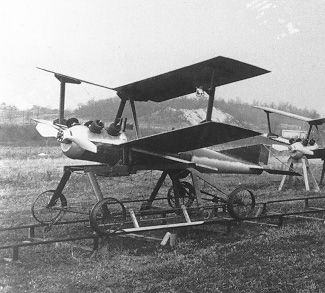
\includegraphics[width=0.5\textwidth]{kettering_bug.jpg}
    \caption{The Kettering Bug (1918)}
    \label{fig:ketteringbug}
\end{figure}

Throughout the 20th century, UAVs become more and more sophisticated, and were used more and more, but always for military purposes. In the more recent years, civilian UAVs have started to appear on the markets and their number quickly exceeded that of military UAVs. In february 2017, the FAA (Federal Aviation Administration) of the United States estimated that around 1.1 million units were in use in the US alone, and expected that number to rise to 3.55 million by 2021 \cite{consumerdronesbythenumbers}. These civilian drones are very different from military drones, in both their form and their function: civilian drones are usually smaller, and use rotors to take off vertically. They are used in a wide variety of applications.

\section{Motivation}
The ability to remote-control small and agile flying objects over large distances through the air, and to bring them to previously inaccessible locations, makes many new things possible. With the increasingly lower prices and better performances of civilian UAVs, people keep finding more and more uses for these high-tech gadgets. Some examples of these applications are: crop monitoring in agriculture \cite{agriculturaldrones}, delivery of mail or parcels, construction \cite{batiravecdesdrones}, cinematography, entertainment, or search and rescue operations. In all these applications, the more autonomous a drone is, the more efficient it will be at its task. One of the main challenges to achieve autonomy is for an UAV to be able to correctly identify its surroundings, and localize itself within them. In outdoor environments, GPS systems allow UAVs to know their position with great accuracy, but this is not possible in GPS-denied environments, such as indoors. The main subject of this thesis will be fully autonomous navigation by a quadcopter in a GPS-denied environment.

\subsection{Ethical considerations}
The new possibilities brought by drones also pose ethical questions about security and privacy. Even though this technology can improve people's quality of life, it also has the potential to diminish it. If drones start to be widely used comercially, we could reach a point where the sound nuisances that they cause seriously impacts people who live in densely populated areas. Also, they can make us feel less at home, knowing that we could be observed from the sky. For this reason, it is important to adopt strict reulations regarding the use of drones in public spaces. Fortunately, many countries are already adopting legislation in this direction.


\section{Context}
This thesis is part of a project at the UCL that spans over several years and several masters theses. This project was launched by professor Julien Hendrickx in the 2012-2013 academic year, and had as long-term goal to develop a program that would enable low-cost UAVs to navigate autonomously in indoor environments. This means creating a map of their environment, localizing themselves in this map, and avoidig obstacles during exploration, using only on-board sensors. Another goal is to allow several drones to collaborate to speed up exploration. Five theses have already been written on this subject, each taking the work of the previous a little further.
\paragraph{2012-2015: First three theses}
In each of the three academic years (2012-2013, 2013-2014, 2014-2015), one masters thesis on the subject of indoor navigation for autonomous low-cost drones was written. These masters theses formed the base of the future work. They implemented visual SLAM methods to allow drones to build a two-dimensional map based on keypoints (first red pucks, then visual landmarks that the drone detected from a textured field of view), and to localize itself within this map. During this time, inter-drone communication was also established, and was used to allow a drone to communicate the location of a target to another drone.

\paragraph{2015-2016: Recent work}
Last year, two groups of students simultaneously wrote theses on this subject. Before doing so, they joined forces to reimplement what had been done previously, but using the ROS interface, an interface to work with robots that would make many things simpler, and allow more flexibility (see section %%TODO for more).
The work of the first group of students allowed a drone to search and follow a mobile target, and call a second drone to continue this task when its battery was low.\\
The second group of students extended to SLAM algorithm to allow to use a 3D map to localize the drone. Unfortunately, they did not implement triangulation to allow to project seen points into 3D space, but rather made the assumption that all points were located on the ground when building the map. The end result was a drone capable of using a 3D map to localize itself, but not capable of building one from its observations.


\section{Objectives}
For my own thesis, my goal is to continue the work of last year's second group, to allow true 3-D SLAM: to build a 3D map based on observations by the monocular camera. To achieve this goal I will follow the following steps:
\begin{itemize}
\item Research the current state of the art for 3D Keyframe based monocular visual SLAM
\item Implement a way to triangulate points based on observations
\item Bundle Adjustment
\item Dense reconstruction
\item Obstacle Avoidance
\end{itemize}

\section{Structure}
%TODO after the rest is done


\chapter{State of the art}
%% State of the art (chpt2)
\section{Multicopters}

\section{Computer Vision}

\section{Simultaneous Localization And Mapping}
Simultaneous Localization and Mapping (SLAM) refers to the joint task of creating a map of a robot's surroundings, while also keeping track of the robot's location in this map. The word "robot" should be understood very broadly in this context, for example it could be a simple handheld camera. Because there are countless different types of robots that do SLAM, SLAM is also a very diverse field, with different algorithms for different kinds of sensors. Here, we will focus on monocular visual SLAM, which is SLAM where the main sensor is a monocular camera.

\subsection{Localization}

\subsection{Mapping}

\section{Bundle Adjustment}


\chapter{Hardware and software architecture}
%%Hardware and software architecture (chpt3)
\section{Hardware}
For this project I used Parrot's AR.Drone 2.0. This quadrotor was commercialized in 2012 and is an updated version of the original AR.Drone that was launched in 2010. This drone was marketed as a high tech toy, and is designed to be controlled from a smarphone application (connected to the drone via Wi-Fi). A few augmented reality games are available for the AR.Drone, in which it can recognise some predefined tags using computer vision, and interact with abject or other drones with a tag. To encourage the creation of more games for their drones, Parrot has released an open SDK that allows to effectively reprogram the drones. This early release of an open SDK has made it quite popular in the scientific community to do research on autonomous flight. The drone consists of 4 rotors, each with their own electric motor and microcontroller, an internal computer with a 1GHz ARM Cortex A8 processor and 1GB DDR2 RAM at 200MHz, and various sensors.

\subsection{Sensors}
Tha AR.drone has the following sensors:
\begin{itemize}
  \item 3 axis accelerometer with $\pm 50$ mg accuracy
  \item 3 axis gyroscope with $\pm 2000\degree/s$ accuracy
  \item Pressure sensor with $\pm 10 \texttt{Pa}$ accuracy
  \item 3 axis magnetometer with $\pm 6\degree$ accuracy
  \item Ultrasound sensor (facing downwards)
  \item Frontal camera (HD 720p 30fps)
  \item Ventral camera (QVGA, 60 fps)
\end{itemize}


\section{Software}

\subsection{Parrot SDK}
The SDK released by Parrot allows to send commands and receive information from the drone. However, it does not allow acces to the lowest-level parts of the drone. It is possible to send the drone commands to take off, land, emergency stop, hover, move in a certain direction, but not to directly control the command send to the motors. Similarly,


\subsection{ROS}


\chapter{Localization}
%%Localization (chpt4)


\chapter{Mapping}
%% Mapping (chpt5)
\section{Triangulation}
\subsection{Bundle Adjustment}


\chapter{Map Initialization}
%Map Initialization (chpt 6)
A robot needs a map lo localize itself within it, but it needs to know its position to find the postion of surrounding objects and build a map. Because the mapping and localization tasks are mutually dependent on one another, there needs to be a special procedure to build a map from nothing when it does not exist yet. Arbitrarily, we decide that the position of the drone when it starts flying is the origin (in all 6 degrees of freedom) of the map. However, with only a monocular camera, it is not possible to find the exact location of any visual features from one observation only, views from at least two different positions are needed to triangulate points.
\section{Procedure}
To reach the position from which the drone will take a second view and triangulate points, the drone has to fly blindly. Blindly here means without using a map la localize itself visually, but the drone can still use its other sensors (IMU and ultrasonic sensor) to obtain an estimate of its postion. Because the ultrasonic sensor is much more accurate than the IMU, and gives an absolute measure, we will mostly rely on this sensor to estimate the relative position from where we take the second view. Because the ultrasonic sensor only gives the distance from the bottom of the drone to the ground, the drone should fly straight up from its first position (the origin) to reach its second position.\\
Once in its second position, the drone can match seen keypoints from both views, and from its estimated position, triangulate those points to the map. However, the drone's estimation of its pose is prone to errors, especially as it only used its ultrasonic sensor and IMU. There errors can be corrected with the information from the cameras, because of we have %TODO how many
matching observations, we can compute the fundamental matrix, and know exactly the displacement between the two views. Refining the poses of the views and the location of the landmarks simultaneously such as to minimize the reprojection error is a nonlinear optimization problem known as Bundle Adjustment. Using Bundle adjustment, we can refine the position of the second view, and use the ultrasonic sensor information to fix the scale. Another advantage of Bundle Adjustment is that it allows to take into account more than 2 views of a point.
\section{Tuning the Bundle Adjustment}
The main drawback of Bundle Adjustment is that it requires an iterative method to be solved and can take a lot of time, which of course is a limiting factor for a robot that builds a map in real time. Therefore it is important to optimize both the speed of the computations, and their precision. As is often the case, there will have to be a tradeoff between these two. To measure both the speed of the Bundle Adjustment and the accuracy of the map obtained, we will conduct some experiments using different parameters to initialize the map.
\subsection{Experimental setup}
We will conduct two different finds of experiments: one to measure the accuracy, and one to measure the robustness of the mapping method. In both cases, we begin by placing the drone at the corner of a desk (position A on figure \ref{fig:benchmarksetup}). After the drone has saved its view, it is placed on a stool exactly above its first position. Its exact pose is then manually communicated to the drone to simulate the measurements from its IMU and ultrasonic sensor. The drone then again takes a snapshot of its camera input, and matches points with the first view, and then adjusts its second pose and the position of the points through bundle adjustment. The drone and stool are then moved to the left (position B on fiugre \ref{fig:benchmarksetup}), and again manually given its exact position, after which it takes another snapshot, matches points with the first two views, and readjusts the poses of the keyframes anf the positions of the points through bundle adjustment. This entire process is rpeated a third time when the drone is placed on the desk again at position D. The initialization of the map consists in making these four keyframes and adjusting their position and that of the landmarks 3 times. After this initialization is done, we place the drone at different locations, and measure how close it is to where it thinks it is. We evaluate the initialization based on how accurate its position estimation is, as well as on how much time the successive bundle adjustments took.
\begin{figure}[H]
  \centering
  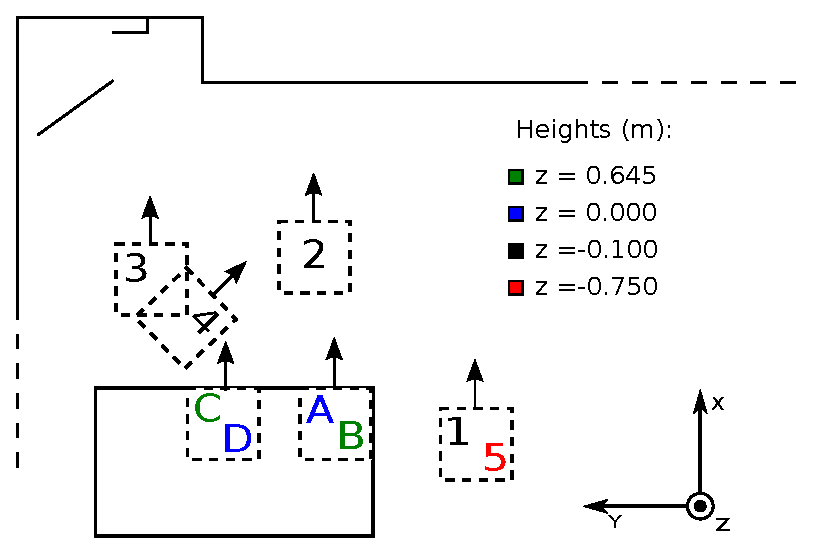
\includegraphics{benchmark_setup.eps}
  \label{fig:benchmarksetup}
  \caption{Different positions of the drone during the validation}
\end{figure}


\chapter{Simultaneous Localization and Mapping}
%Simultaneous Localization and Mapping (chpt 07)

\subsection{Loop Closure}



%%Alternative: contraire: 3D Slam, reconstruction, pathplanning, avec subsections implementation, performance

\chapter{Conclusion}
%%Conclusion (chpt6)


\printbibliography

\appendix
\chapter{Appendix Title}
\chapter{Full code flowchart}\label{app:flowchart}
\begin{figure}[H]
\centering
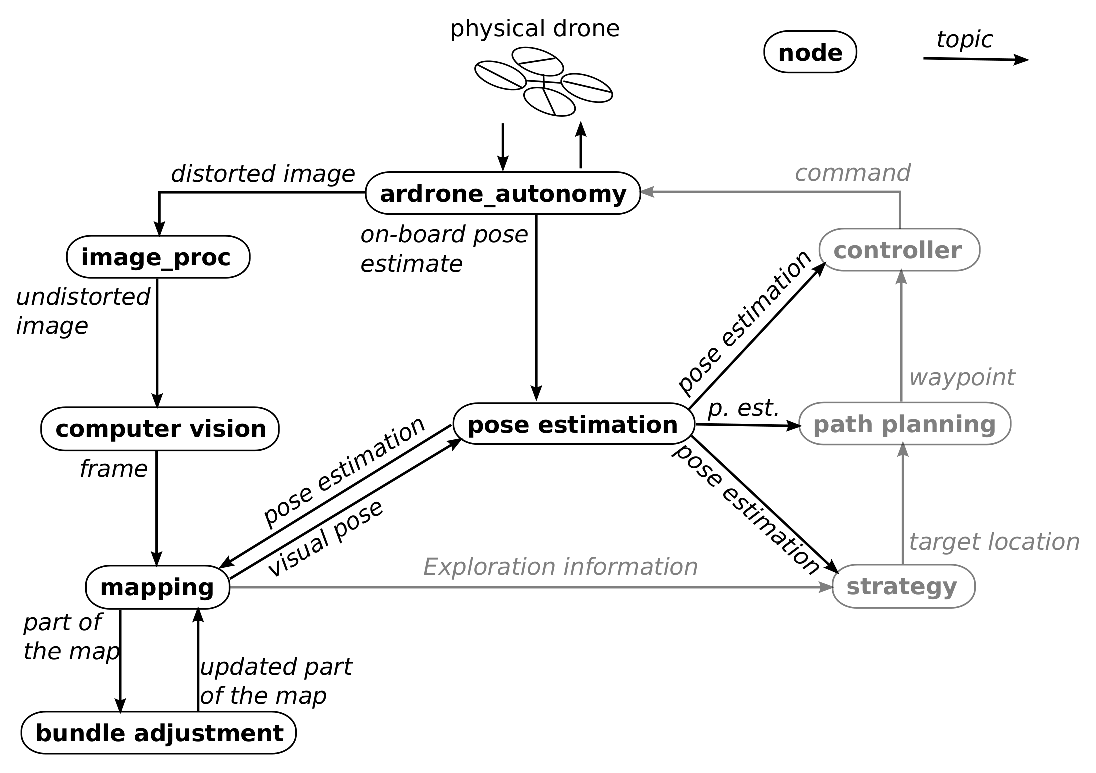
\includegraphics[width=\linewidth]{flowchart.eps}
\caption{Flowchart of the different nodes and the communication between them. Grayed-out parts were not worked on in this master's thesis}
\label{fig:fullflowchart}
\end{figure}


% Back cover page
%\backcoverpage

\end{document}
